%liste des modules réalisés
%Preuve du fonctionnement de chaque modules

\subsection{Taxonomie}%Martin
Nous avons rencontrés deux problème majeurs avec cette technique.
D'abord, le temps d'execution de cette méthode pour un seul document sur le texte en entier dépassait largement les limites de l'acceptable.
En effet, un document administratif est presque par nécessité très verbeux, et donc long. La majorité du texte ne nous est cependant pas utile pour notre but; 
il ne sert qu'à donner du contexte pour le lecteur et ne donne pas forcément d'information concernant le sujet du document en lui même. 

Deuxièmement, nous n'avons pas pu obtenir les résultats escomptés.
Le principal obstacle venant du fait que les mots de la taxonomie peuvent être en fait des phrases, ou tout du moins de multiples mots dont les sens ne sont pas forcément corrélés.
On trouve par exemple "amménagement foncier", mais aussi "fromage au lait cru" ou bien encore "médecine physique et de réadaptation".
La technique que nous utilisions pour obtenir les \textit{embeddings}, word2vec, ne fonctionne pas sur des \textit{groupes de mots} ou \textit{n-grammes}, mais sur des mots seuls.
Doc2vec, qui lui peut fonctionner sur des n-grammes, voires des paragraphes ou documents entier a besoin d'être entrainé sur des documents qui lui apporteront le contexte nécessaire pour former des \textit{embeddings} correct.
Cependant, la taxonomie ne donne aucun contexte.
Il s'agit seulement d'une liste de mot et de phrase ordonnée seulement sous la forme d'un arbre.
Il ne s'agit pas d'un document ordinaire, et nous pouvions pas utiliser les techniques courantes dans ce cas. 

Pour essayer de contrer ce problème, la décision initale fut de transformer chaque mot de la phrase en sa racine par le procédé de la lemmatization a l'aide de la librairie spacy\cite{spacy} et d'enlever les \textit{stopwords} de la phrase.
Les \textit{stopwords} sont des mots apparant très fréquement dans les phrases, comme les déterminants.
Ainsi la phrase "médecine physique et de réadaptation" se trouve transformée en "médecine physique réadaptation".
On utilise ensuite un word2vec sur chaque mot pour obtenir plusieurs vecteurs. Pour obtenir un seul vecteur que nous comparerons avec les mots du documents, nous effectuons un simple moyennage.
Cependant, cette solution n'as pas fonctionné et les taxonomies que nous trouvions a l'aide de ce système ne correspondait simplement pas au document. 

La solution finale adaptée fut celle de simplement extraire les titres d'arrétées administratifs, qui sont les documents a classer, et a les prétraiter par lemmatization et élimination des stopwords avant d'effectuer une simple recherche dans la taxonomie.
Si un mot de la taxonomie se trouve dans le titre de l'article administratif, alors celui ci est ajouté au document.
Cette solution est non seulement bien plus simple et permet de vérifier la qualité des résultats plus aisément qu'à l'aide d'un \textit{embedding}, et elle est de plus bien plus rapide, permettant l'analyse d'un document entier en quelques secondes à peine contre plusieurs minutes a l'aide d'un word2vec.

\begin{figure}[h!]
  \centering
  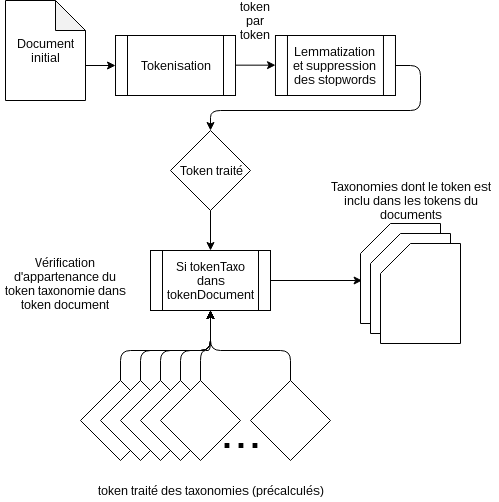
\includegraphics[width=0.8\textwidth]{diagFinalTaxo.png}
	\caption[]{Schéma fonctionnel du module d'assignement taxonomique final}
  \label{taxoFinal}
\end{figure}

On notera que le système final n'utilise pas d'apprentissage.
On peut y voir ici une piste d'amélioration: avec un corpus de données annotés, il devient trivial de construire un module taxonomique plus précis et performant, car prenant en compte le contexte, crucial dans le NLP.
En effet, notre système ne peut distinguer "outre mer" de "mer". Si ces deux exemples contiennent le mot "mer", il est évident que leur sens sémantique est différent.
Ce sens ne peut être compris que par le contexte; fonctionnalité qui manque a ce module. 
